\documentclass[tikz,margin=0pt,dvipsnames,rgb]{standalone}

\usepackage{amsmath,amssymb,amsfonts}
\usetikzlibrary{calc,
fit,
shapes.misc,
shapes.geometric,
arrows.meta,
fadings,
matrix,
chains,
scopes,
positioning}

\usepackage{pgfplots}
\usepackage{pgfplotstable}
\pgfplotsset{compat=1.18}



\usepackage[]{fontspec}

\setmainfont{Latin Modern Roman}
\setmonofont{Latin Modern Math}
\renewcommand{\textsc}[1]{{\fontfamily{lmr}\selectfont \scshape #1}}

\usepackage[]{bm}

\makeatletter
\@ifundefined{fromRoot}{\newcommand{\fromRoot}[1]{../../#1}}{}

\def\input@path{{../..}{..}{.}{./svg}{./pgfplots}{./tikzpicture}}
%or: \def\input@path{{/path/to/folder/}{/path/to/other/folder/}}
\makeatother

\newcommand*{\gf}[1]{\acrshort{gf}($#1$)}%
\newcommand*{\mpn}[1]{\bm{P}_{#1}}%
\newcommand*{\pn}[1]{%
  \ifthenelse{\equal{#1}{}}{$\mpn{0}$}{$\mpn{#1}$}%
}%

\newcommand*{\pk}[3]{%
  \ifthenelse{\equal{#1}{#2}}{\textcolor{red}{\phantom{.}$p_0$\phantom{.}}}{\phantom{.}$p_#3$\phantom{.}}%
}%


\newcommand*{\placeholder}{
\includegraphics[width=\linewidth, height=.25\textheight, keepaspectratio = true]{figures/certified_xilinx.png}}%

\newcommand*{\snr}{\acrshort{snr}}%
\newcommand*{\snrs}{\acrshortpl{snr}}%

\newcommand*{\mpd}[0]{p_\Delta}%
\newcommand*{\mpo}[0]{p_\omega}%
\newcommand*{\pd}[0]{$\mpd$}%
\newcommand*{\po}[0]{$\mpo$}%
\newcommand*{\mpfa}[0]{\mathcal{P}_{fa}}%
\newcommand*{\mpmd}[0]{\mathcal{P}_{md}}%
\newcommand*{\pfa}[0]{\acrshort{pfa}}%
\newcommand*{\pmd}[0]{\acrshort{pmd}}%
\newcommand*{\mnorm}[1]{\mathcal{L}_{#1}}%
\newcommand*{\norm}[1]{$\mnorm{#1}$}%
\newcommand*{\fft}{\acrshort{fft}}%
\newcommand*{\mfft}[1]{\mathcal{F}(#1)}%
\newcommand*{\mifft}[1]{\mathcal{F}^{-1}(#1)}%
\newcommand*{\ts}{\acrshort{ts}}%

\newcommand*{\cpp}[1]{C\textrm{++#1}}%
\newcommand*{\na}{\textrm{\textcolor{SlateGray4}{N/A}}}%

\newcommand*{\vect}[1]{\bm{#1}}%
\newcommand*{\mat}[1]{\bm{\mathrm{#1}}}%

\newcommand*{\task}[1]{\mathcal{T}_{#1}}%

\newcommand*{\sdr}{\acrshort{sdr}}%
\newcommand*{\fpga}{\acrshort{fpga}}%



\begin{document}
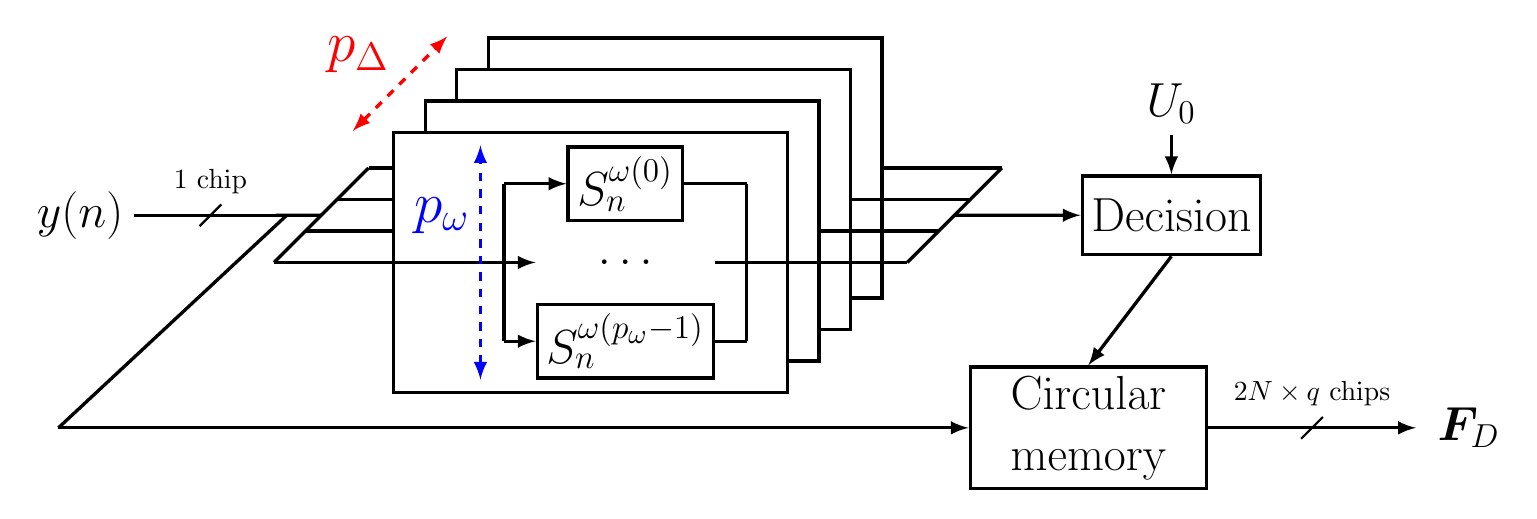
\begin{tikzpicture} [-latex,
    >=latex,
    auto,
    very thick,
    every node/.style={font=\LARGE},
    main node/.style={rectangle, fill = white!35, draw, align=center}]

  \node [] (yn) at (0, 0) {$y(n)$};

  \node [right = 1.8cm of yn ] (pack) {};

  \draw [-] (yn) -> (pack.center)
  node [midway, anchor=center, label={above:\normalsize $1$ chip}] (ttt) {};
  \draw [-, thick] (ttt.north east) -- (ttt.south west);

  \node [draw = none,
    fill = none,
    minimum size = 2cm,
    minimum width = 3.2cm,
    right = 2.7 cm of pack
  ] (anchor_ccskd) {};

  % \draw [-] (pack.east) -> ($(anchor_ccskd.west) + (-1.5, 0)$)
  % node [pos=1, align=center] (pack_mid) {};

  % \draw (pack_mid.south) -> ($(anchor_ccskd) + (0, 4.5cm)$)
  % node [midway, align=center] (pack_mid) {};

  \def \a{.4}
  \foreach \len in {3,2,1,0}{
      \node [main node,
        % fill = gray!40!white, 
        minimum size = 3.3cm,
        minimum width = 5cm
      ] (pcd\len) at ($(anchor_ccskd) + (\len * \a, \len * \a) + (-.6, -.6)$) {};

      \draw [-] ($(pcd\len.west) + (-1.5, 0)$) -- (pcd\len.west);
      \draw [-] (pcd\len.east) -- ($(pcd\len.east) + (1.5, 0)$);
      % \draw ($(pcd\len.west) + (-1.8, -1.5)$) -- ($(pcd\len.west) + (-1.5, 0)$);
    }

  \draw [-] ($(pcd0.west) + (-1.5, 0)$) -- ($(pcd3.west) + (-1.5, 0)$)
  node [midway, right] (point_west) {};
  \draw [-] ($(pcd3.east) + (1.5, 0)$) -- ($(pcd0.east) + (1.5, 0)$)
  node [midway, left] (point_east) {};

  \draw [-] (pack.west) -> (point_west);


  % \node [main node,
  %   % fill = gray!40!white, 
  %   minimum size = 2cm,
  %   minimum width = 3.2cm
  % ] (pcd0) at (anchor_ccskd) {};

  % \node [draw = red,
  %   fill = none,
  %   minimum size = 1.8cm,
  %   minimum width = 3.5cm
  % ] (frame_ccskd) at (anchor_ccskd) {};

  \node [main node,
    % fill = gray!40!white,
    minimum size = 1cm,
    % minimum width = 2cm,
    right = 4cm of anchor_ccskd
  ] (dec) {Decision};

  \node [above = .5cm of dec] (U0) {$U_0$};
  \draw (U0.south) -- (dec.north);

  \draw [->] (point_east) -> (dec.west);

  \node [] (pbuf) at ($(pack.center) + (-2.9, -2.7)$) {};

  \draw [-] (pack.center) -- (pbuf.center);

  \node [ main node,
    minimum width = 3cm,
    align = center,
    % minimum width = 10cm,
    %below = 2cm of anchor_ccskd
  ] (buf) at ($(pbuf -| dec.west) + (.1,0)$) {Circular\\memory};

  \draw (pbuf.center) -- (buf);

  \draw (dec.south) -- (buf.north);

  \node [
    right = 2.5cm of buf,
    align = center,
    label= {right:$\vect{F}_D$}
  ] (out) {};

  \draw (buf.east) -- (out.center)
  node [midway, anchor=center, label={above:\normalsize $2 N \times q$ chips}] (ttt) {};
  \draw [-, thick] (ttt.north east) -- (ttt.south west);

  \node[main node,
    %minimum size = 1cm,
    anchor=west
  ] (fcd3) at ($(pcd0) + (-.7, -1)$) {$S^{\omega(p_\omega - 1)}_n$};

  \node[
    minimum width = 1.5cm,
    % anchor=west
  ] (fcd2) at (pcd0 -| fcd3.center) {$\ldots$};

  \node[main node,
    %minimum size = 1cm,
    % anchor=west
  ] (fcd1) at ($(pcd0 -| fcd3.center) + (0, 1)$) {$S^{\omega(0)}_n$};

  \draw ($(fcd3.west |- fcd1.west) + (-.4,0)$) -- (fcd1.west);
  \draw [-] (fcd1.east) -- ($(fcd3.east |- fcd1.east) + (.4,0)$);

  \draw (pcd0.west) -- (fcd3.west |- pcd0);
  \draw [-] (fcd3.east |- pcd0) -- (pcd0.east);

  \draw ($(fcd3.west) + (-.4,0)$) -- (fcd3.west);
  \draw [-] (fcd3.east) -- ($(fcd3.east) + (.4,0)$);

  \draw [latex-latex, dashed, red] ($(pcd0.north west) + (-.5, 0)$) -- ($(pcd3.north west) +  (-.5, 0)$)
  node [midway, font={\huge}] (n_p) {$p_\Delta$};

  \draw [latex-latex, dashed, blue] ($(fcd3.south west) + (-.7,0)$) -- ($(fcd3.south west |- fcd1.north west) + (-.7,0)$)
  node [pos=.7, font={\huge}] (n_f) {$p_\omega$};

  \draw [-] ($(fcd3.west) + (-.4,0)$) -- ($(fcd3.west |- fcd1.west) + (-.4,0)$);

  \draw [-] ($(fcd3.east) + (.4,0)$) -- ($(fcd3.east |- fcd1.east) + (.4,0)$);

  % \draw [-] (pcd0.west) -- ($(pcd0.west) + (.5,0)$);

\end{tikzpicture}

\end{document}
